\documentclass{llncs}
\usepackage{times}
\usepackage[T1]{fontenc}

% Comentar para not MAC Users
\usepackage[applemac]{inputenc}

\usepackage{a4}
%\usepackage[margin=3cm,nohead]{geometry}
\usepackage{epstopdf}
\usepackage{graphicx}
\usepackage{fancyvrb}
\usepackage{amsmath}
%\renewcommand{\baselinestretch}{1.5}

% CAPITAL LETTER LETTRINE
\usepackage{lettrine}

\begin{document}
\mainmatter
\title{Overview of Content-Delivery Networks Architecture}

\titlerunning{Paper Title}

\author{Afonso Silva\and Alfredo Gomes \and Axel Ferreira}

\authorrunning{Autor1 \and Autor2 \and Autor3}

\institute{University of Minho, Department of Informatics, 4710-057 Braga, Portugal\\
e-mail: \{a70387,a71655,a53064\}@alunos.uminho.pt
}

\date{\today}

\bibliographystyle{splncs}
%---------------- TITLE
\maketitle

%---------------- TABLE OF CONTENTS
%\tableofcontents
%\newpage



%%%%%%%%%%%%%%%%%%%%%%%%%%%%%%%%%%%%%%%%%%%%%%%%%%%%%%%%
%---------------- ABSTRACT							%(Axel)
%%%%%%%%%%%%%%%%%%%%%%%%%%%%%%%%%%%%%%%%%%%%%%%%%%%%%%%%
\begin{abstract}
Given the diversity of existing Content Delivery Networks (CDN) architectures and the lack of a reference explicitly organising this information, this paper intends to overview three main CDN architectures. A description of Traditional Commercial \textit{CDN}s, Peer-to-Peer (P2P) \textit{CDN}s and Hybrid \textit{CDN}s is presented. For each architecture, the advantages, disadvantages, technical challenges and application scopes are presented.
Implications for further research and practice are discussed.
\end{abstract}
%----------------



%%%%%%%%%%%%%%%%%%%%%%%%%%%%%%%%%%%%%%%%%%%%%%%%%%%%%%%%
\section{Introduction}									%(Axel)
%%%%%%%%%%%%%%%%%%%%%%%%%%%%%%%%%%%%%%%%%%%%%%%%%%%%%%%%
%According to Table~\ref{tab:TabelaExemplo} \dots

%\subsection{Context}
\lettrine[lines=2]{T}{he} Internet has its origins in the early 1980's and presented an exponential growth when commercial companies started to link to the existing academic and military networks during the 90's. As the popularity of the Internet increased the number of devices connected started to see an exponential growth.\\ 
% \subsection{Problems }
At that time networks were unreliable and Internet communication protocols were designed in a robust fashion. As an example, Hypertext Transfer Protocol (HTTP) was designed to survive multiple packet losses and thus being a very chatty protocol, there are multiple Round-trip Time (RTTs) this causes a latency problem over long distance communication.
Modern networks are faster and more reliable, but most of the core protocols mentioned above don't take advantage of the increased reliability. %(Due to Backwards compatibility)
As the Internet role in daily life grew, new technologies star to emerge providing images videos and other dynamic content. This caused a bottleneck in servers with popular content.
The above problems, led to the development Content Delivery Networks.

%\subsection{What is a \textit{CDN}?}
A Content Delivery Network ( \textit{CDN}) is a large network of distributed storage servers which cash the content in multiple locations strategically spread. Traditionally \textit{CDN} servers are stored in ISP's facilities. This reduces both infrastructural costs to \textit{CDN} Providers and ISP's costs by keeping popular content local, in contrast to bringing it from another ISP's network.

%\subsection{How does it Work?}
A \textit{CDN} works by keeping a copy of the content in different locations. Whenever content is requested, management software calculates the best Server for accessing the content. This reduces distance to server which improves latency and minimizes packet loss. 
Since the calculations are dynamic, in case of a server malfunction another Server is chosen, providing redundancy.
%\subsection{ \textit{CDN} Service vs in House Solution}
Traditional \textit{CDN} business model target bandwidth as a cost factor. This brings two advantages over a 'In House' solution:
First, there are no initial infrastructural costs, this is a big advantage. An example of the dimension of such structure's size would be Akamai's infrastructure. It is composed by more than 61,000 servers, spread across 1000 networks in 70 countries worldwide\cite{akamai};
Second, provides bandwidth on demand. In comparison with an 'In House' solution, there is no need to deal with both predictable and unpredictable traffic peaks.
Due to its large distributed infrastructure, and high bandwidth on demand \textit{CDN}s are especially well suited to absorve a Denial of Service (DoS) attacks\cite{cdnetworks}.

%\subsection{Costs}
It is worth noting that \textit{CDN}s bring cost per performance down. Despite that, \textit{CDN}s are expensive, and currently are used mostly by big companies. It is imperative that \textit{CDN}'s get cheaper. This will allow more parties to use them, thus enhancing Internet experience to the final consumer and reducing total Internet traffic at the same time.
% Exemplo (åmbito de aplica‹o) Netflix
An example of a service using a \textit{CDN} (Amazon EC2) would be the popular movie streaming service Netflix.


\subsection{Purpose} %Prop—sito do paper
This paper's purpose is to provide organised information about different \textit{CDN} architectures: the traditional large server infrastructure \textit{CDN}, the Peer to Peer (P2P) \textit{CDN} and a new trend of Hybrid architecture which relies on both Servers and Peers. 






%%%%%%%%%%%%%%%%%%%%%%%%%%%%%%%%%%%%%%%%%%%%%%%%%%%%%%%%
\section{Academic \textit{CDN} (P2P)}						%(Afonso)
%%%%%%%%%%%%%%%%%%%%%%%%%%%%%%%%%%%%%%%%%%%%%%%%%%%%%%%%

As said before \emph{CDN Commercial Architecture} brings mostly advantages to clients but it comes with high financial cost. This
happens due to the large distributed infrastructure that causes expensive
financial cost of server renting. Therefore only big companies like \emph{Akamai}
(leading company in this area) can afford it, making de \textit{CDN} market very
centralised and consequently making the fees associated with the service
really high. As a result, small and medium sized Internet content providers
are not allowed to grow because they are not in a financially viable position
to rent the services of commercial \textit{CDN} providers. Only large firms can
afford it.


In order to improve this big disadvantage another architecture was implemented:
the \emph{Academic Architecture}.

\subsection{Aplication Scope}

In contrast to commercial architectures, \emph{academic} (P2P) ones are free, both in terms of profit and advertisement. \emph{peer-to-peer} architectures, where each user shares a some of their machine's resources (Storage, CPU cycles, \dots) with the remaining
peers. 
In other words, P2P architecture creates a distributed storage medium that facilitates the search, the publishing and recovery of files by members of the network.

\subsubsection{Main Advantages}

This alternative makes the network independent from ??entrepreneurial?? servers,
which makes it significantly cheaper (the price to pay is the small shared resources).

Another advantage of this architecture comes from the increased quality and speed
of the network in proportion to the number of users, i. e., the more users it has,
the faster and the more reliable it becomes. 
For instance, high quality streaming to a great number of users may benefit from
using an \emph{academic architecture}, as the provider of that same stream won't
have to deal with the cost of renting a server and, beyond that, the high number
of users will guarantee a wide array of available resources to a global video
transmission.

\subsection{Associated Challenges}
Despite being better,when it comes to costs,
than the previous option, it still has some disadvantages.
The biggest disadvantage is that availability and quality of the content
reception depends on content providers that are volunteers and therefore don't
follow a clear set of rules causing a lack of standard specification of
\textit{CDN} interfaces.
Consequently, this makes it hard to maintenance and support end users.






%%%%%%%%%%%%%%%%%%%%%%%%%%%%%%%%%%%%%%%%%%%%%%%%%%%%%%%%
\section{Hybrid \textit{CDN} Architecture}					%(Alfredo)
%%%%%%%%%%%%%%%%%%%%%%%%%%%%%%%%%%%%%%%%%%%%%%%%%%%%%%%%

As it has been shown, both \emph{comercial} architecture and 
\emph{academic} architecture present some drawbacks that may 
??make unviable?? it's utilisation in medium scale. If on one hand,
\emph{commercial} architecture has it's cost only viable for 
large scale aplications, on the other hand the \emph{academic}
one is dependant on the number and quality of it's \emph{peers}
which can cause some instability and lack of sturdy.
In this way, it becomes central to look for more reliable alternatives
that can combine \emph{the best of both worlds}. A currently already
proposed architecture is the ``Distributed Content Delivery Networks''
\texttt{D \textit{CDN}}, which is an hybrid model that is between 
\emph{comercials} and \emph{academics} \textit{CDN}.




\subsection{Aplication Scope}

\subsubsection{Framework}
The \texttt{D \textit{CDN}} are composed by a well defined hierarchical structure
that allows a better relationship among the network's elements.
This way, it is possible to defined to following entities (from higher
to the lower level of the hierarchy):

% Talvez fosse importante p™r a imagem que est‡ no paper,
% d‡ para perceber muito melhor a hierarquia e a distribui‹o
% de conteœdo nem que fosse para a apresenta‹o

\begin{itemize}
\item \textbf{Content provider} - creator and manager of the shared content;

\item \textbf{Administrators} - a group of users with privileges on the 
network responsible for the network's maintenance and support

\item \textbf{Servers} - a set of servers, that are utilized, not to
data storage, but for the efficient distribution of network content.
They can be \emph{Master} tipe (directly connected to the
\emph{content provider}, distributing the content by the various regions
where the \textit{CDN} acts) or \emph{Local} (connected to the 
\emph{master servers} andchannel the content to the \emph{surrogates}
acting on a closer level to the client).

\item \textbf{Surrogates} - set of users of P2P network whose
resources are shared;

\item \textbf{Client} - final entity, that gets the content;

\end{itemize}



\subsubsection{Content Distribution Method}

Given that the main point of \texttt{D \textit{CDN}} is to optimize the content acess
and minimize it's costs, it makes sense that the content replicas
are as close as possible to the client, i.e., on the \emph{surrogates}.
This way, content distribution is made sequentially in the following way:
\begin{enumerate}

\item The \emph{content providers} ask permission to 
\emph{administrators} to insert a new content on the network;

\item If the request is successful, \emph{master} servers send
the updated content to the \emph{local} servers and from them to 
the \emph{surrogates};

\item At the same time that the content is sent, servers update their
records with the same contents being that the \emph{master} will own more general data
(like the network area where the content is distributed) 
and the \emph{local} more specific informations (i.e, that \emph{surrogates}
are in possession of the contents);

\item When there is an content access request by the 
\emph{client}, the \emph{local} server will choose the valid \emph{surrogates}
for the content share. This way, this is distributed between the
\emph{surrogates} and the \emph{client} through the \emph{peer-to-peer} network.
\end{enumerate}



\subsubsection{Main Advantages}

The main advantage of this architecture, when compared to the \emph{comercial},
is it's reduced cost of implementation (because there is a need 
of much less servers).

When compared to the \emph{academic} architecture, this model assures a
better content stability and availability, for it does not depend 
only on the volunteer \emph{peer-to-peer} effort. 

With this architecture becomes also possible to restrict the content
with the client's location, because the content distribution is made
by the \emph{master} and \emph{local} servers. This way, if the 
\emph{content providers} intend that a specific content will only be
accessible from determined place, the content will only be sent to
that region's servers, therefore preventing other region's users
to access it.


\subsection{Associated Challenges}

This architecture has some drawbacks, the main being that this is
only an hypothetical model, with few or none real implementation
and, consequently is a little tested platform.

Relatively to the \emph{academic} and \emph{comercial} \textit{CDN},
the \emph{Distributed CDN (DCDN)} adds some levels of complexity to the structure and
hierarchy, which may difficult it's physical implementation.

Once more, the lack of standards to the \textit{CDN} is also
a drawback that must be deal with as quickly as possible.




%%%%%%%%%%%%%%%%%%%%%%%%%%%%%%%%%%%%%%%%%%%%%%%%%%%%%%%%
\section{Lista de projetos atuais}							%(Alfredo)
%%%%%%%%%%%%%%%%%%%%%%%%%%%%%%%%%%%%%%%%%%%%%%%%%%%%%%%%	

The following list contains the most popular \textit{CDN} service providers. According to \cite{reuters}, Akamai, being the biggest \textit{CDN} provider, and is responsible for as much as 15\%-30\% of the Internet traffic.

Another interesting perspective is to evaluate the offerings available. Most of them are commercial \textit{CDN}s. 


-O paper "Standard IPTV CDN Architecture Interfaces" Fala sobre desafios
		¼ Falta de standards
		¼ Incompatibilidade entre as CDNs existentes (impossibilita a mobilidade)
		%-Lack of standards and Norms => hard to change provider

	
\if
	Cloud Content Delivery Networks
	
		Free CDNs
			BootStrap CDN\\
			CloudFlare\\
			C CDN\\
			Incapsula\\
			\dots\\
		Telco CDN\\
			AT\&T\\
			Verizon\\
			\dots\\
		Traditional CDNs\\
			Akamai\\
				Amazon\\
			Windows Azure\\
			HP Cloud\\
			CloudFlair\\
			\dots 

		Commercial CDN P2P\\
			BitTorrent\\
			Internap\\
			\dots\\
\fi




%%%%%%%%%%%%%%%%%%%%%%%%%%%%%%%%%%%%%%%%%%%%%%%%%%%%%%%%
\section{Conclusion and Future Work}						%(Axel)
%%%%%%%%%%%%%%%%%%%%%%%%%%%%%%%%%%%%%%%%%%%%%%%%%%%%%%%%





nossa perspetiva
-Arquitectura h’brida => Despite the  Further practical testing is needed to take better conclusions

- a contribui‹o œnica Ž o paper focado nos custos gerais em fun‹o das diferentes arquiteturas

-Referir que este paper est‡ limitado ‡ perspetiva da bibliografia


%%%%%%%%%%%%%%%%%%%%%%%%%%%%%%%%%%%%%%%%%%%%%%%%%%%%%%%% 
%--------------- G L O S S A R I O ----------------%		%(Axel)
%%%%%%%%%%%%%%%%%%%%%%%%%%%%%%%%%%%%%%%%%%%%%%%%%%%%%%%%
\if
	CDN - Content-delivery Network
	DCDN - Distributed Content-delivery Network
	DNS - Domain Name System
	RTT - round-trip time
	PoP - Points of Presence
	ASP - Application Service Provider
	SaaS - Software as a Service
	Caching -
	Mirroring -
\fi	
%%%%%%%%%%%%%%%%%%%%%%%%%%%%%%%%%%%%%%%%%%%%%%%%%%%%%%%%
%----------- B I B L I O G R A F I A -------------%			%(Axel)
%%%%%%%%%%%%%%%%%%%%%%%%%%%%%%%%%%%%%%%%%%%%%%%%%%%%%%%%

% Inserir directamente os v‡rios \bibitem 
\begin{thebibliography}{1}
	\bibitem{reuters}
	Anya George Tharakan, Subrat Patnaik: 
	\newblock{"Strong dollar hurts Akamai's profit forecast, shares fall" (http://www.reuters.com/article/2015/04/28/us-akamai-tech-results-idUSKBN0NJ2IV20150428)}

	\bibitem{akamai}
	Erik Nygren, Ramesh K. Sitaraman, and Jennifer Sun.:
	\newblock {"The Akamai Network: A Platform for High-Performance Internet Applications" (ACM SIGOPS Operating Systems Review, vol. 44, no. 3, July 2010)}

	\bibitem{ cdnetworks}
	"How Content Delivery Networks Work" (http://www. \textit{CDN}etworks.com/blog/how-content-delivery-networks-work/).
	Networks. Retrieved 22 September 2015.

	\bibitem{DCDN} % Arquitectura híbrida
	Mulerikkal, J.P. and Khalil, I.:
	\newblock{"An Architecture for Distributed Content Delivery Network" (http://ieeexplore.ieee.org/xpls/icp.jsp?arnumber=4444113)}

	% Exemplo deum BibItem 
	%	\bibitem{Nguyen99}
	%	Nguyen, H., Walker, E.:
	%	\newblock {First course in fuzzy logic}.
	%	\newblock {Boca Raton: Chapman and Hall/CRC Press} (1999)

\end{thebibliography}


%%%%%%%%%%%%%%%%%%%% FIGURAS %%%%%%%%%%%%%%%%%%%%%%%%%%% %(Axel)
%\if
%De acordo com o ilustrado na Figura~\ref{fig:controller}
% Exemplo para inser‹o de uma figura
%\begin{figure}
%\begin{center}
%\includegraphics[scale=0.30]{no \textit{CDN}} 
%\end{center}
%\caption{\label{fig:controller}Architecture of the unified QoS metric fuzzy controller.}
%\end{figure} 

%De acordo com o ilustrado na Figura~\ref{fig:controller}
% Exemplo para inser‹o de uma figura
%\begin{figure}
%\begin{center}
%\includegraphics[scale=0.30]{ \textit{CDN}} 
%\end{center}
%\caption{\label{fig:controller}Architecture of the unified QoS metric fuzzy controller.}
%\end{figure} 

%De acordo com o ilustrado na Figura~\ref{fig:controller}
% Exemplo para inser‹o de uma figura
%\begin{figure}
%\begin{center}
%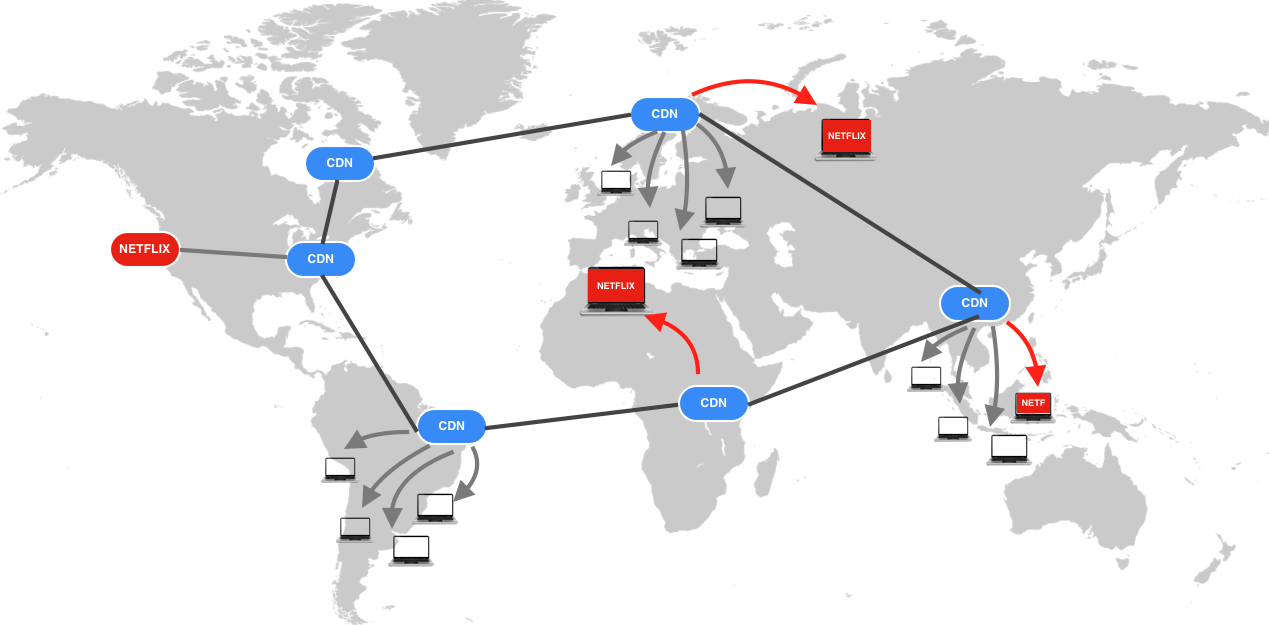
\includegraphics[scale=0.30]{map} 
%\end{center}
%\caption{\label{fig:controller}Architecture of the unified QoS metric fuzzy controller.}
%\end{figure} 
%\fi


\end{document}
